\documentclass{article}[11pt]

\usepackage{amsmath}
\usepackage{amsfonts}

%\usepackage{fullpage}

\usepackage{graphicx}
\graphicspath{{data/}}

\usepackage{pgfplots}
\usepackage{tikz}
\usetikzlibrary{arrows, shapes, fit, decorations.markings}

\tikzstyle{vecArrow} = [thick, decoration={markings,mark=at position
   1 with {\arrow[semithick]{open triangle 60}}},
   double distance=1.4pt, shorten >= 5.5pt,
   preaction = {decorate},
   postaction = {draw,line width=1.4pt, white,shorten >= 4.5pt}]
\tikzstyle{innerWhite} = [semithick, white,line width=1.4pt, shorten >= 4.5pt]

\newcommand{\inputTikZ}[1]{%
  \input{data/#1.tikz}%
}

\newcommand{\TODO}[1]{\emph{\small{{\bf TODO: } #1}}}

\newcommand{\etal}{\textit{et al.}}
\newcommand{\etc}{\textit{etc.}}
\newcommand{\eg}{\textit{e.g.}}


\title{Multi-Sensory Integration : Theories, Empirical Observations and Models}
\author{Weipeng He \\ \texttt{2he@informatik.uni-hamburg.de} \\ \texttt{6411529}}

\begin{document}

\maketitle

\section*{Abstract}
\TODO{abstract}

%\tableofcontents
%\pagenumbering{arabic}
%\clearpage

\section{Introduction}
\label{sec:intro}

Multisensory integration is a process, which is carried out by animals to combine different sensory cues in order to get a better perception of the environment. This process is essential as multi-modal senses provide complementary information.
For example, humans use both visual and haptic information to perceive the size and position of an object \cite{ernst_humans_2002}. Some mammals integrate visual and vestibular information to estimate self-motion \cite{gu_visual_2006}.

Multisensory integration is also involved in some interesting phenomena. One of these phenomena is the ventriloquist effect \cite{alais_ventriloquist_2004}. The effect comes from a performance art -- ventriloquism, in which the performer makes his/her voice appear to come from elsewhere. The audience may feel that the sound is from the puppet, of which the mouth is moving. This effect results from vision ``capturing'' sound.
Another phenomenon is the stream/bounce illusion \cite{sekuler_sound_1997}. An experiment was conducted, where a video of two oscillating circles was given and subjects may have two ambiguous perception : either the circles stream pass each other or they collide and bounce apart. The interesting fact is that, when simply adding a click sound, more subjects reported that they perceived the circles as bouncing apart.

In order to explain these intriguing phenomena, researchers from a variety of disciplines try to analyze the nature of multisensory integration from different aspects. According to their methods, the studies of understanding multisensory integration are divided into two approaches -- psychophysical approach and neurophysiological approach.

\begin{figure}[htpb]
  \centering \inputTikZ{flow}
  \caption{The procedure of multisensory perception and the analysis levels of different study.}
  \label{fig:flow}
\end{figure}

These two approaches study multisensory integration in different levels (see Figure \ref{fig:flow}).
Figure \ref{fig:flow}a is an illustration of how multisensory perception is processed in levels. Stimuli of two different modalities are perceived and processed separately by primary unisensory neurons. Following this, sensory information are integrated by a population of multisensory neurons. Finally, the results of the multisensory neurons are further interpreted and, then, exhibited by behaviors.

As depicted in Figure \ref{fig:flow}b, the psychophysical study of multisensory integration analyzes the behavioral responses of multisensory input. Usually, in psychophysical experiments, human subjects are given sensory input and asked to do discrimination tasks. The behavior of subjects are observed. An example of this is the psychophysical study of the ventriloquist effect, in which the human localization of different visual and auditory input is tested \cite{alais_ventriloquist_2004}.

Whereas the psychophysical study ignores the intermediate neural precesses in brain areas, the neurophysiological study investigate the neural basis of multisensory integration (see Figure \ref{fig:flow}c). Techniques, like neuron recording and brain imaging, are used to observe the neuronal responses (firing rate) of multisensory neurons.

Additional to difference in analysis levels, these two approaches also differ in directions of research. The psychophysical study is from theory to observation. At first, a theory of what mathematical model is optimal (normative prediction) is studied. Then, behaviors observed are compared to the normative prediction. On the contrary, the neurophysiological study first measures the neuronal responses in related brain areas and corresponding computational models are proposed next. A number of empirical principles are established according to the physiological observations \cite{stein_merging_1993, stanford_evaluating_2005}.

As both approaches have significant achievements, it is particularly interesting to study how these approaches relate to each other. The following questions have been raised (as depicted as a question mark in Figure \ref{fig:flow}): \emph{How are the neuronal responses related to behaviors? What are the computational rules of multisensory neurons? Are these rules consistent with normative predictions?} 

% Recent studies have answered these questions \cite{fetsch_bridging_2013}.

The purpose of this paper is to try to answer these questions. This paper first briefly reviews the key findings of both psychophysical and neurophysiological studies of multisensory integration. Afterwards, a study that relates these two approaches is introduced. Finally, a neural network model that accounts for these findings is outlined.

\section{Theories and psychophysics of multisensory integration}
As was pointed out in the introduction to this paper, psychophysical study of multisensory integration involves theoretical deduction and behavioral observation.

Considering multisensory perception as a mathematical problem, there are numerous discussions about the computational and statistical solution to the problem. The problem, which is called optimal cue integration, is that, given several cues with uncertainties, what is the optimal estimate by combining these cues together. A solution to the problem is called an ideal observer model. Depending on the assumptions of the uncertainty of the source cues and what the observer is trying to optimize, there is a variety of ideal observer models being proposed \cite{landy_ideal-observer_2011}.

With the theoretical support of optimal cue integration, recent psychophysical experiments found out that multisensory perception of humans as well as primates closely matches the optimal prediction \cite{ernst_humans_2002,alais_ventriloquist_2004,fetsch_neural_2012}.

\subsection{Linear model for maximum reliability}
A simple linear ideal observer model is successful in predicting the optimal estimate under certain assumptions. This model is one of the standard models for testing multisensory behavior \cite{landy_ideal-observer_2011}.

The set-up of the model is that, the system get multiple source cues ($\hat{S}_i, i=1 \dots n$) with different reliability ($g_i$), which is decided by the variance($\sigma_i$), as input. Then the best estimate ($\hat{S}_{opt}$) is given by the weighted sum of all cues, where the weights ($w_i$) are proportional to the reliability of the corresponding cues:
\begin{gather}
  \hat{S}_{opt} = \sum_{i=1}^{n} w_i \hat{S}_i \label{eq:optest} \\
  w_i = \frac{g_i}{\sum_{i=1}^{n} g_i}, \quad g_i = \frac{1}{\sigma_i^2} \label{eq:optweight}
\end{gather}
and the optimal estimate has a higher reliability ($g_{opt}$) than that of any input cues:
\begin{equation}
  g_{opt} = \sum_{i=1}^{n} g_i \label{eq:optrel}
\end{equation}

With simplifying assumptions, this estimation is in accord with Bayesian inference \cite{knill_bayesian_2004}. According to Bayes' theorem, the posterior probability of the real value ($X$) under condition of two observations ($C_1, C_1$) is:
\begin{equation}
  P(X|C_1,C_2) = \frac{P(C_1,C_2|X)P(X)}{P(C_1,C_2)}
\end{equation}
If one assumes independent Gaussian noise, that is Gaussian distribution of the two observations, and a uniform prior, the probability is:
\begin{equation} \label{eq:post}
  P(X|C_1,C_2) \propto P(C_1|X)P(C_2|X)
\end{equation}
This product is also a Gaussian of which the mean and inverse of variance are consistent to Equation \ref{eq:optest} and \ref{eq:optrel} respectively.

\begin{figure}[htpb]
  \centering \inputTikZ{bayes}
  \caption{Example of standard linear ideal observer model.}
  \label{fig:bayes}
\end{figure}

Figure \ref{fig:bayes} is an illustration of how the ideal observer model combines two sensory cues. The two cues (depicted as green and blue curves) are normally distributed around different centers ($\hat{S}_1$ and $\hat{S}_2$). The combined estimate, which is calculated by Equation \ref{eq:post}, is shown as the red curve. By using information from both cues, the combined estimate has higher reliability (the height of the curve).

\subsection{Behavioral experiments}
The linear ideal observer model combines sensory cues in a statistically optimal fashion. Surprisingly, a number of psychophysical experiments have shown that humans process multisensory cues in an analogous way. These experiments examined human visual-haptic integration \cite{ernst_humans_2002} and audio-visual integration \cite{alais_ventriloquist_2004}.

\begin{figure}[htpb]
  \centering
  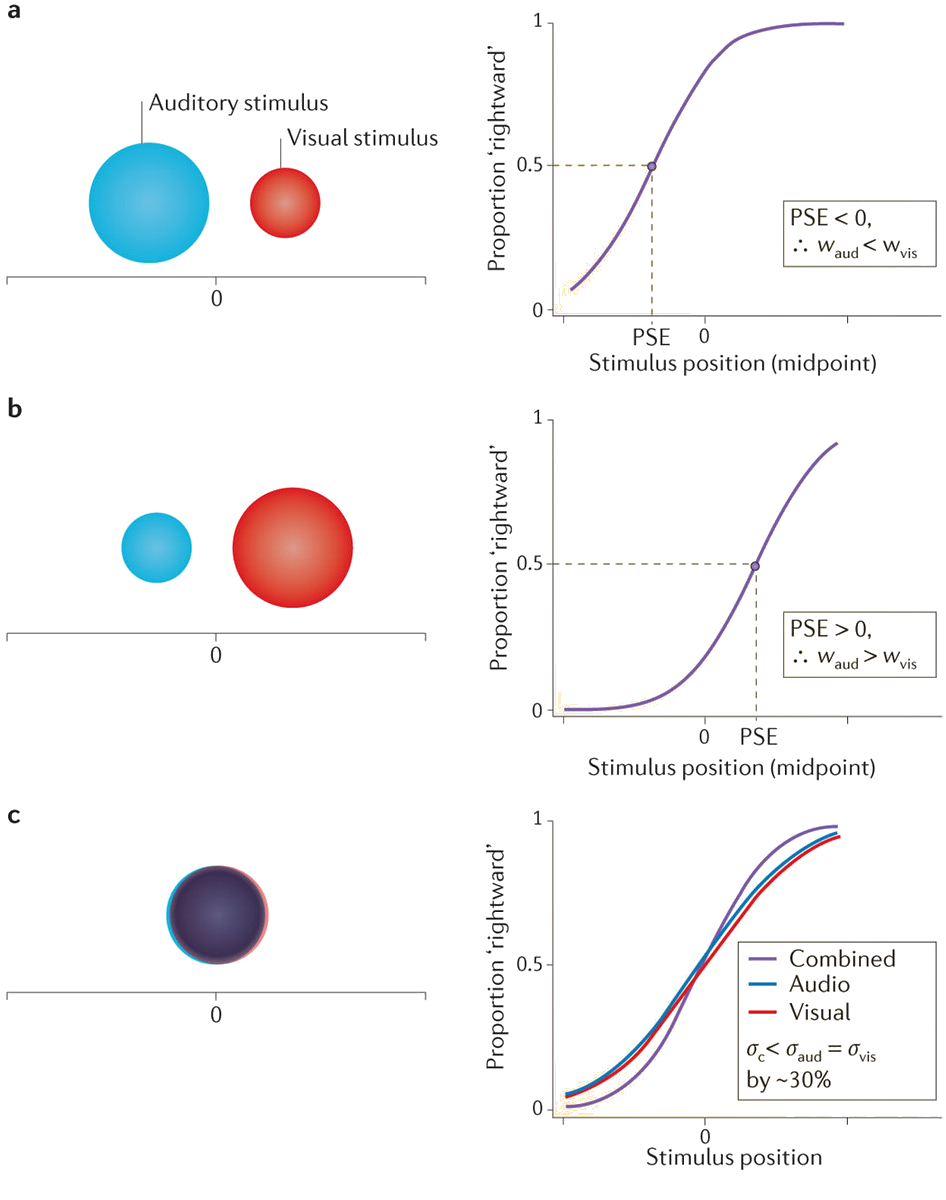
\includegraphics[width=.9\textwidth]{fetsch-visaudloc}
  \caption{Behavioral experiments of visual and auditory localization task. (from \cite{fetsch_bridging_2013})}
  \label{fig:visaudloc}
\end{figure}

One of the experiments \cite{alais_ventriloquist_2004} carried out simple spatial localization tasks, in which subjects were given visual and auditory stimuli and asked to report whether the stimuli were from left or right. Both visual and auditory stimuli were controlled in position and reliability. The result is shown in Figure \ref{fig:visaudloc}.

In the first experiment (Figure \ref{fig:visaudloc}a), the two modal of stimuli were in conflict position, where the visual stimulus was displaced on the left. Also the visual stimulus was more reliable (depicted by smaller circle) than the auditory stimulus. With the midpoint of the stimuli changed from left to right, the proportion of subjects choosing right increased from 0 to 1. As shown in the figure, the point of subjective equality (PSE), where subjects have equal tendency of left and right, is smaller than 0. This indicates that the visual cue, which is more reliable, dominates the auditory cue.

In the second experiment (Figure \ref{fig:visaudloc}b), after changing the reliability of the visual stimulus to less than that of the auditory stimulus, the PSE shifted to larger than 0. This also indicates that the more reliable cue is given higher weight, which is in accord with Equation \ref{eq:optweight}.

In the third experiment (Figure \ref{fig:visaudloc}c), the performance of multisensory cue integration was compared against unisensory cue. The visual and auditory stimuli were placed in congruent position with same reliability. The right figure shows that the curve of combined cumulative Gaussian psychometric function has steeper slope than that of unisensory cue. In addition, data show that the standard deviation of combined cue decreased by $30\%$. This is approximate to $1-\sqrt{2}$, which we can calculate using optimal cue integration (Equation \ref{eq:optweight} and \ref{eq:optrel}).

The result indicates that humans perform near-optimally in multisensory perception. It is interesting to note that humans have the ability to adapt to the changing of reliability of cues (by modifying the weight in Equation \ref{eq:optest}). Additionally, experiments also shows that primates also have the similar performance in vision-vestibular integration \cite{fetsch_neural_2012}.

\section{Neurophysiology of multisensory integration}
In parallel to psychophysical studies, neuroscientists try to explain multisensory integration phenomena on account of the neural basis.
They use neurophysiological recording or brain imaging to examine the physiological properties of a neuron or a population of neurons that underlies the integration functions.

Multisensory neurons are found in many brain areas, including superior colliculus \cite{stein_merging_1993} and cortex (posterior parietal area \cite{graziano_system_2001} and superior temporal area \cite{alais_multisensory_2010}).
Among all neurophysiological studies, there are two groups of influential work -- the classical multisensory studies in cat superior colliculus \cite{stein_merging_1993, stein_multisensory_2008} and a recent body of work on vision-vestibular integration in primate dorsal medial superior temporal area \cite{gu_visual_2006, morgan_multisensory_2008, fetsch_dynamic_2009, fetsch_visualvestibular_2010}.
In the former studies, some key principles of sensory integration are established. The later studies focus on reliability-based cue weighting and linking the physiological evidence to behavioral observations.

%Researchers found that multisensory neurons are particularly abundant in the superior colliculus (SC), a midbrain structure primarily involved in orienting the eyes and head towards salient stimuli \cite{sparks_translation_1986}. Another area in brain that caught interest from researchers is the dorsal medial superior temporal area (MSTd), which is responsible for integration visual and vestibular cues for detecting self-motion \cite{gu_visual_2006}.

\subsection{Multisensory integration in SC and empirical principles}
By studying the cat SC area for multisensory integration, researchers found a number of empirical principles, which state the properties of multisensory integration \cite{meredith_interactions_1983}. The most prominent principles are the ``inverse effectiveness'' and ``spatial and temporal principle''.

\TODO{details about ``inverse effectiveness'' and ``spatial and temporal principle''.}

\subsection{Development of multisensory integration}
Besides understanding the usage of multisensory integration, plentiful of researches are into knowing how multisensory integration is acquired. 

\TODO{a short overview of physiological study of development of MSI.}

\section{Neural network models}
With the insight from psychophysical and physiological study, a number of computational models, including neural network models are developed. 

\subsection{The normalization model}
Among all computational models of multisensory integration, the normalization model \cite{ohshiro_normalization_2011} is of particular interest. This model helps to explain several key empirical findings: the reliability-dependent combination rule in area MSTd as well as
the empirical principles that were initially described in classic studies of the SC.

\TODO{details of normalization model.}

\subsection{}
\TODO{other models.}

\section{Discussion}
\TODO{summarize current achievement; discuss how these studies can give insight to develop more practical models (artificial systems ?)}

\addcontentsline{toc}{section}{References}
\bibliography{bib}
\bibliographystyle{unsrt}

\end{document}
